% DesertMap model card. Build from the repo root:
%   uv run python docs/model_card/make_assets.py && tectonic docs/model_card/model_card.tex
% Every data number comes from numbers.tex, generated from site/data/summary.json.
\documentclass[10pt,letterpaper]{article}

\usepackage[letterpaper,left=0.55in,right=0.55in,top=0.5in,bottom=0.62in,footskip=0.3in]{geometry}
\usepackage{fontspec}
\setmainfont{SourceSansPro}[
  Extension=.otf, UprightFont=*-Regular, BoldFont=*-Semibold,
  ItalicFont=*-RegularIt, BoldItalicFont=*-SemiboldIt]
\newfontfamily\headfont{SourceSansPro}[Extension=.otf, UprightFont=*-Bold]
\setmonofont{SourceCodePro}[Extension=.otf, UprightFont=*-Regular, Scale=0.9]
\usepackage{microtype}
\usepackage[dvipsnames]{xcolor}
\usepackage{graphicx}
\usepackage{booktabs}
\usepackage{multicol}
\usepackage{enumitem}
\usepackage[skins]{tcolorbox}
\usepackage{titlesec}
\usepackage{caption}
\usepackage{fancyhdr}
\usepackage{hyperref}

% Colors: deep teal accent, darker teal for text on white; red for risk.
\definecolor{accent}{HTML}{0F766E}
\definecolor{accentdark}{HTML}{115E59}
\definecolor{accentwash}{HTML}{F0FDFA}
\definecolor{risk}{HTML}{DC2626}
\definecolor{riskwash}{HTML}{FEF2F2}
\definecolor{ink}{HTML}{1F2937}
\definecolor{muted}{HTML}{4B5563}
\definecolor{rulegray}{HTML}{D1D5DB}
\color{ink}

\hypersetup{
  colorlinks=true, linkcolor=accentdark, urlcolor=accentdark,
  pdftitle={DesertMap Model Card}, pdfauthor={Morgan Anunda},
  pdfsubject={Model card for the DesertMap food-desert classifier and its fairness audit},
  pdfkeywords={model card, fairness audit, food deserts, HOLC, redlining, random forest, SHAP}}

\newcommand{\best}[1]{\textbf{\color{accentdark}#1}}
% Generated by make_assets.py from site/data/summary.json. Do not edit.
\newcommand{\NTracts}{72{,}531}
\newcommand{\NMapped}{72{,}506}
\newcommand{\FoodDesertShare}{12.8\%}
\newcommand{\ImbalanceRatio}{6.8}
\newcommand{\HolcRatio}{1.53}
\newcommand{\HolcRatioTest}{1.30}
\newcommand{\HolcLabelRatio}{1.82}
\newcommand{\CdRate}{20.3\%}
\newcommand{\AbRate}{13.3\%}
\newcommand{\HolcN}{16{,}421}
\newcommand{\FairFOne}{0.533}
\newcommand{\FairFOneNoRace}{0.486}
\newcommand{\FairDeltaPts}{4.7}
\newcommand{\FlipRate}{16.4\%}
\newcommand{\FprDisparity}{3.5}
\newcommand{\ShapIncomeShare}{43\%}
\newcommand{\ShapPovertyShare}{27\%}
\newcommand{\ShapRaceShare}{8\%}
\newcommand{\HolcRateA}{8.8\%}
\newcommand{\HolcRateB}{14.9\%}
\newcommand{\HolcRateC}{19.4\%}
\newcommand{\HolcRateD}{21.8\%}
\newcommand{\RfFOne}{0.533}
\newcommand{\LrFOne}{0.438}
\newcommand{\RfFOneCell}{\best{0.533}}
\newcommand{\LrFOneCell}{0.438}
\newcommand{\RfPrec}{0.446}
\newcommand{\LrPrec}{0.302}
\newcommand{\RfPrecCell}{\best{0.446}}
\newcommand{\LrPrecCell}{0.302}
\newcommand{\RfRec}{0.661}
\newcommand{\LrRec}{0.800}
\newcommand{\RfRecCell}{0.661}
\newcommand{\LrRecCell}{\best{0.800}}
\newcommand{\RfAuc}{0.885}
\newcommand{\LrAuc}{0.838}
\newcommand{\RfAucCell}{\best{0.885}}
\newcommand{\LrAucCell}{0.838}


% Layout
\setlength{\parindent}{0pt}
\setlength{\parskip}{3.2pt}
\setlength{\columnsep}{0.28in}
\linespread{1.04}
\frenchspacing
\setlist{nosep, leftmargin=1.05em, topsep=1pt, itemsep=1.6pt}
\setlist[enumerate]{leftmargin=1.25em}
\titleformat{\section}{\headfont\fontsize{10.5}{12}\selectfont\color{rulegray}}{}{0pt}{\textcolor{accentdark}}[\vspace{1.5pt}\titlerule]
\titlespacing*{\section}{0pt}{8pt}{1pt}
\captionsetup{font={footnotesize,color=muted}, labelfont={bf,color=muted}, labelsep=period, skip=2pt, justification=raggedright, singlelinecheck=false}
\newcommand{\lbl}[1]{\textbf{#1}\enspace}

\pagestyle{fancy}
\fancyhf{}
\renewcommand{\headrulewidth}{0pt}
\fancyfoot[L]{\footnotesize\color{muted}DesertMap Model Card \textbullet{} November 2026}
\fancyfoot[R]{\footnotesize\color{muted}Page \thepage{} of 2}

\begin{document}

% ==== header band
\begin{tcolorbox}[enhanced, sharp corners, boxrule=0pt, toprule=3pt,
  colframe=accent, colback=accentwash, left=10pt, right=10pt, top=6pt, bottom=6pt]
{\headfont\fontsize{21}{24}\selectfont DesertMap Model Card}\par\vspace{2pt}
{\fontsize{11.5}{14}\selectfont A Random Forest food-desert classifier for \NTracts{} US census tracts, with a four-part fairness audit.}\par\vspace{4pt}
{\small\raggedright\color{muted}\textbf{Version} November 2026 \quad\textbullet\quad \textbf{Author} Morgan Anunda\\ \href{https://github.com/Morgan971-pixel/desertmap}{github.com/Morgan971-pixel/desertmap} \quad\textbullet\quad \href{https://desertmap.vercel.app}{desertmap.vercel.app}\par}
\end{tcolorbox}

\vspace{1pt}
% ==== key finding
\begin{tcolorbox}[enhanced, sharp corners, boxrule=0.8pt, colframe=accent, colback=white,
  sidebyside, sidebyside align=center, lefthand width=1.25in, segmentation hidden,
  left=8pt, right=10pt, top=5pt, bottom=5pt]
\centering{\headfont\fontsize{34}{36}\selectfont\color{accentdark}\HolcRatio\texttimes{}}\par
{\footnotesize\color{muted}\textbf{KEY FINDING}}
\tcblower
The model flags tracts in formerly redlined neighborhoods (HOLC grades C and D) as food deserts at \textbf{\HolcRatio{} times the rate} of A- and B-graded tracts: \CdRate{} against \AbRate. It never saw a HOLC grade; it rebuilt the 1930s map from present-day income, poverty and demographic data, so any use of its predictions inherits that history unless someone audits for it. Actual food desert rates differ by \HolcLabelRatio\texttimes{} between the same grades, so the gap is real and the model tracks it.
\end{tcolorbox}

\vspace{2pt}
\raggedcolumns
\begin{multicols}{2}

% ==== model details
\section*{Model details}
\begin{itemize}
  \item \lbl{Model} scikit-learn Random Forest tuned by 3-fold grid search on F1: 200 trees, max depth 20, min split 5, class-balanced weights. Baseline: logistic regression.
  \item \lbl{Task} Binary classification of \texttt{LILATracts\_1And10}, the USDA flag for a tract that is low income and low access (a large share of residents more than 1 mile from a supermarket if urban, 10 miles if rural).
  \item \lbl{Inputs (9)} Median family income; poverty rate; \% Black, \% Hispanic and \% White population; \% households with no vehicle; \% SNAP households; total population (2010); urban flag. No HOLC grades, ZIP codes or place names.
  \item \lbl{Explanations} SHAP (TreeExplainer) scores how far each feature pushed each tract's prediction.
\end{itemize}

% ==== intended use
\section*{Intended use}
Research and teaching: a worked example of how a model trained on current data can inherit historical discrimination, and of the audit that catches it. Analysts can also use it to explore tract-level food access, reading each prediction beside its SHAP explanation and the audit below.

\textbf{Out of scope}
\begin{itemize}
  \item Allocating funding, stores or services to individual tracts without a fresh audit and threshold calibration.
  \item Causal claims. The model estimates neither what causes food deserts nor the effect of redlining.
  \item Judging individual households; labels describe whole tracts.
  \item Other countries, or years far from 2019, without retraining.
\end{itemize}

% ==== data
\section*{Data}
\begin{itemize}
  \item \lbl{Source} USDA ERS Food Access Research Atlas 2019, all \NTracts{} tracts on 2010 census geography. \FoodDesertShare{} are food deserts.
  \item \lbl{Split} 80/20, stratified on the label, seed 42: 58,024 training and 14,507 test tracts.
  \item \lbl{Preparation} Shares derived from tract counts; continuous features capped at the 1.5\,\texttimes\,IQR fences.
  \item \lbl{Audit only} HOLC crosswalk from Mapping Inequality v3 (Nelson et al., 2023), joined to 2010 tracts: \HolcN{} tracts graded A to D. We used it only to group finished predictions.
\end{itemize}

% ==== metrics
\section*{Metrics}
Held-out test set, food-desert class. F1 is the primary metric because positives are rare.

\vspace{2pt}
{\centering\small
\begin{tabular}{@{}lcccc@{}}
\toprule
Model & F1 & Precision & Recall & ROC-AUC \\
\midrule
Random Forest & \RfFOneCell & \RfPrecCell & \RfRecCell & \RfAucCell \\
Logistic regression & \LrFOneCell & \LrPrecCell & \LrRecCell & \LrAucCell \\
\bottomrule
\end{tabular}\par}
\vspace{3pt}
{\footnotesize\color{muted}Bold teal marks the better model on each metric. Test-set metrics from the November 2026 re-run (scikit-learn 1.9).}

The forest leads on F1, precision and ROC-AUC. The baseline finds more true food deserts (recall \LrRec) but raises far more false alarms (precision \LrPrec).

% ==== fairness audit
\section*{Fairness audit}
Four checks, each built to test a different route by which race could enter the predictions.
\begin{enumerate}
  \item \lbl{F1 ablation} Refitting without the three race shares drops F1 from \FairFOne{} to \FairFOneNoRace{} (\FairDeltaPts{} points). Race shares carry signal that income and poverty do not replace.
  \item \lbl{Quartile FPR} Across quartiles of \% Black, the top quartile's false positive rate is \textbf{\FprDisparity\texttimes{}} the bottom one's.
  \item \lbl{Counterfactual probe} Setting all three race shares to their held-out median, all else fixed, flips \textbf{\FlipRate} of held-out food-desert predictions to ``not a food desert''.
  \item \lbl{HOLC overlay} C- and D-graded tracts are predicted food deserts at \textbf{\HolcRatio\texttimes{}} the A+B rate. This is a ratio of rates (\CdRate{} over \AbRate); the rate climbs with every grade from A to D. Held-out tracts alone give \HolcRatioTest\texttimes; true labels give \HolcLabelRatio\texttimes.
\end{enumerate}
{\footnotesize\color{muted} All four checks use the tuned model above. Checks 1 and 3 remove or reset \% Black, \% Hispanic and \% White together, since the shares sum to nearly 100\% and any one reveals the others. Checks 1 to 3 use the held-out test set; check 4 covers all \NTracts{} tracts, training tracts included.}

% ==== subgroups
\section*{Subgroups examined}
We broke results out by \% Black quartile, \% Hispanic quartile and HOLC grade. The Hispanic pattern differs from the Black one: false positives barely change across quartiles (11\% to 13\%), and the most Hispanic quartile has the lowest recall, so there the model tends to miss real food deserts (test set). The audit has no urban versus rural or regional breakdown yet, and rural tracts are where the Atlas data is thinnest.

\begin{center}
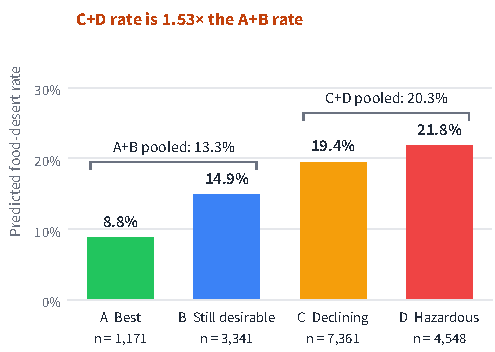
\includegraphics[width=\linewidth]{fig_holc.pdf}
\captionof{figure}{Predicted food-desert rate by HOLC grade (\HolcN{} graded tracts). HOLC is the Home Owners' Loan Corporation, a federal agency that graded neighborhoods in over 200 cities between 1935 and 1940; grade D went predominantly to Black and immigrant neighborhoods, and the maps shaped where banks lent.}
\end{center}

% ==== global drivers
\section*{Global drivers}
\begin{center}
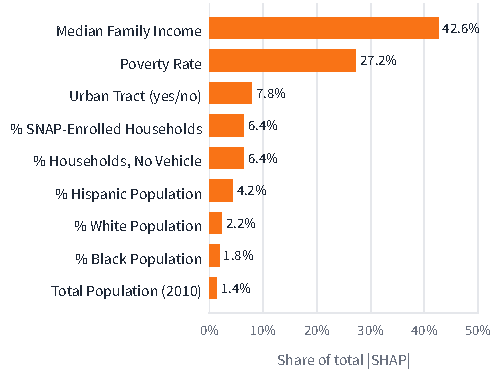
\includegraphics[width=\linewidth]{fig_shap.pdf}
\captionof{figure}{Each feature's share of summed absolute SHAP values, counted over every tract's top three drivers (\NMapped{} mapped tracts).}
\end{center}
A longer bar means the feature moved more predictions further; the chart shows size of influence and leaves out direction. Income and poverty dominate (\ShapIncomeShare{} and \ShapPovertyShare). The three race shares add up to \ShapRaceShare, with \% Hispanic in sixth place. Rank understates effect: the counterfactual probe still flips one in six positive predictions.

SHAP values exist for every tract, and the website shows each tract's three strongest drivers so a reviewer can check any single prediction. Values come from path-dependent TreeSHAP and add up to each tract's predicted probability.

\columnbreak
% ==== limitations
\begin{tcolorbox}[enhanced, sharp corners, boxrule=0pt, leftrule=3pt, colframe=risk, colback=riskwash,
  left=7pt, right=7pt, top=4pt, bottom=5pt, before skip=8pt, after skip=4pt]
{\headfont\fontsize{10.5}{12}\selectfont\color{risk}LIMITATIONS AND RISKS}\par\vspace{2pt}
\begin{itemize}
  \item \lbl{Observational} The audit shows association. It cannot say that redlining caused today's food deserts, or that race causes the model's errors.
  \item \lbl{Race as input} \% Black, \% Hispanic and \% White are model inputs. We kept them so the audit could measure their effect; any deployment must justify that choice or drop them (removing all three cost \FairDeltaPts{} F1 points).
  \item \lbl{Capped features} IQR capping means model inputs differ from raw census shares in extreme tracts.
  \item \lbl{Dated geography} 2019 data on 2010 tract boundaries. The HOLC overlay covers only surveyed cities, mostly older Northern and Midwestern ones.
  \item \lbl{Imbalance} About \ImbalanceRatio{} negatives per food desert. At precision \RfPrec, most flagged tracts are false alarms.
  \item \lbl{Proxy label} The USDA flag measures supermarket distance and income. It misses corner stores, markets, and time or transport barriers.
\end{itemize}
\end{tcolorbox}

% ==== ethics
\section*{Ethical considerations}
Food-access labels steer grants and store siting. A biased model could send resources away from, or stigmatize, the neighborhoods redlining already harmed, so we publish the disparity with the model. Before any real use we recommend store-level distance data, per-quartile thresholds that narrow the false positive rate gap (equalized odds or threshold adjustment), uncertainty reported with every prediction, and ongoing monitoring of false positive rates by quartile.

% ==== reproduce
\section*{Reproduce}
{\raggedright Code, data pipeline and notebooks live at \href{https://github.com/Morgan971-pixel/desertmap}{github.com/\allowbreak Morgan971-pixel/\allowbreak desertmap}. Run \texttt{uv sync}, then notebooks 01 to 06 in order, then:\par}
\vspace{1pt}
{\footnotesize\ttfamily uv run python scripts/export\_static\_data.py\\
uv run python docs/model\_card/make\_assets.py\\
tectonic docs/model\_card/model\_card.tex}\par
\vspace{2pt}
{\footnotesize\color{muted}Format follows Mitchell et al., ``Model Cards for Model Reporting'' (FAT* 2019).}

% ==== terms
\section*{Terms}
\begin{itemize}
  \item \lbl{Census tract} A small, neighborhood-sized area the US Census Bureau uses for statistics.
  \item \lbl{Precision} Of the tracts the model flags, the share that really are food deserts.
  \item \lbl{Recall} Of the real food deserts, the share the model flags.
  \item \lbl{F1} The harmonic mean of precision and recall, so a model cannot score well by trading one away.
  \item \lbl{ROC-AUC} The chance the model ranks a random food desert above a random non-desert; 0.5 is a coin flip.
  \item \lbl{False positive rate} The share of non-desert tracts the model wrongly flags.
  \item \lbl{SHAP} Splits one prediction into per-feature contributions, using Shapley values from game theory.
\end{itemize}

\end{multicols}
\end{document}
